\documentclass[12pt]{report}
\usepackage[utf8]{inputenc}
\usepackage[myheadings]{fullpage}

% Package for headers 
\usepackage{fancyhdr}
\usepackage{lastpage}
\usepackage{titlesec}
  
% For figures and stuff
\usepackage{graphicx, wrapfig, subcaption, setspace, booktabs}
\usepackage[T1]{fontenc}

% Change for different font sizes and families
\usepackage[font=small, labelfont=bf]{caption}
\usepackage{fourier}
\usepackage[protrusion=true, expansion=true]{microtype}

%% line and paragraph spacing
% \linespread{1.0}
\setlength{\parskip}{1em}
% \titlespacing{\section}{0pt}{2.5ex plus 1ex minus .2ex}{1.3ex plus .2ex}

% Maths
\usepackage{amsmath,amssymb}
\usepackage{float}
\usepackage{graphicx}
\usepackage{wrapfig}
\usepackage[colorinlistoftodos]{todonotes}
\usepackage[colorlinks=true, allcolors=blue]{hyperref}

% % Bibliography
\usepackage{biblatex} 
\addbibresource{references.bib}

%% Language and font encodings
\usepackage[english]{babel}

% % code
% Better inline directory listings
\usepackage{listings}
\usepackage{xcolor}
\definecolor{light-gray}{gray}{0.95}
\newcommand{\code}[1]{\colorbox{light-gray}{\texttt{#1}}}
\definecolor{codegreen}{rgb}{0,0.6,0}
\definecolor{codegray}{rgb}{0.5,0.5,0.5}
\definecolor{codepurple}{rgb}{0.58,0,0.82}
\definecolor{backcolour}{rgb}{0.95,0.95,0.92}

\lstdefinestyle{mystyle}{
    backgroundcolor=\color{backcolour},   
    commentstyle=\color{codegreen},
    keywordstyle=\color{magenta},
    numberstyle=\tiny\color{codegray},
    stringstyle=\color{codepurple},
    basicstyle=\ttfamily\footnotesize,
    breakatwhitespace=false,         
    breaklines=true,                 
    captionpos=b,                    
    keepspaces=true,                 
    % numbers=left,                    
    % numbersep=5pt,                  
    showspaces=false,                
    showstringspaces=false,
    showtabs=false,                  
    tabsize=4
}

\lstset{style=mystyle}

\newcommand{\HRule}[1]{\rule{\linewidth}{#1}}
\onehalfspacing
\setcounter{tocdepth}{5}
\setcounter{secnumdepth}{5}

%% Sets page size and margins
\usepackage[a4paper,top=2cm,bottom=1.5cm,left=2cm,right=2cm,marginparwidth=1.5cm]{geometry}

% Enable header and footer 
\pagestyle{fancy}
\fancyhf{}

% Header and footer information
\setlength\headheight{15pt}
\fancyhead[L]{ECE 5725 \- Lab1} 
\fancyhead[R]{Yu Zhang\quad Xinyu Wu}
\fancyfoot[R]{\thepage}

\setlength{\parindent}{0pt} 

\begin{document}

\date{}

% Do not change anything here except in \LARGE \textbf{This is the title of the essay} 
% /hline before and after the title makes those horoziontal lines appear, you can change the appearance by changing the 2pt to different sizees
\title{ \normalsize {\textbf{Cornell University}}
		\\ [1.0cm]
		% Change to your faculty if needed
		
\includegraphics[width=25mm]{img/cornell_logo.png}\\[.5cm]
		Electrical & Computer Engineering \\
		\HRule{2pt} \\
		\LARGE \textbf{ ECE 5725 Embedded Operating System} \\%para que quede encerrado en las lineas
		\LARGE {\color{blue}{\textbf{LAB1 Report}}}
		\HRule{2pt} \\ [0.5cm]
		\normalsize \ {Lab Section: \textbf{Thursday} }\\
% 		\normalsize \today \vspace*{5\baselineskip}
		\normalsize \ {Lab Date: 09/09/21 \And 09/16/21} \vspace*{5\baselineskip}\\
		}
		
\author{
		{ \textbf{Yu Zhang (yz2729)}} \quad \&  \quad {Xinyu Wu (xw586)}\\[5cm]
		\large {\textbf{\today} } 
		}
		

\maketitle
%\newpage

% Uncomment the next line if you want keywords/index terms after the abstract. 
%\textit{\textbf{Keywords}: lorem, ipsum, dolor}
\section*{1. Introduction\vspace{-1em}}
In the lab1, We obtained the initial knowledge of Raspberry Pi and the Linux operating system. The main topic is to let us learn how to setup the Raspberry Pi with a piTFT display, play videos on the piTFT display by applying the \code{myplayer} application and write Python scripts to control the video playing with the \code{FiFO} file and physical buttons on the piTFT display. We successfully completed all the parts and were always the first team to demonstrate the result to the TA in this lab section.\vspace{-1em}
\section*{2. Design and Testing\vspace{-1em}}
In this section, we will introduce our experimental process step by step and describe in detail the phenomena and problems we encountered, the solutions and the final results.
\subsection*{2.1 \quad Assemble the Raspberry Pi and  Setup the Linux System\vspace{-1em}}
As mentioned in the first section, the first aim of this lab is to assemble the Raspberry Pi kit with a piTFT display and setup the Linux system. To be honest, this part was very convoluted and much harder than we expected. \par
First, we followed the steps in the manual and quickly assembled the Raspberry Pi with all required cable connected except plugging the power. But when we confidently showed the professor the finished work, the professor pointed out that we had assembled it wrong as the white stripe was installed in the opposite direction. According to the manual, the white strip on the cable should be positioned next to the small "1" on the pin side which is also the direction that the buttons are located. But even though we knew this mistake, it was still hard for us to pull it out by our hands. finally a TA used a screwdriver to help us slowly warp it out. The final assembled Raspberry Pi with the piTFT display is shown in the figure \ref{fig:fig1}. (The photo was taken after the lab.)\par
\begin{figure}[H]
    \includegraphics[width=8cm, height = 8cm]{img/Figure1.png}
    \centering
    \caption{Properly assembled Raspberry Pi and piTFT display}
    \label{fig:fig1}
\end{figure}
We had got a less-than-stellar start, but the rest of the process was not smooth either.\par
After booted to the system, we firstly run some commands to get some system information for checking if the system is installed correctly. The commands included \code{whoami}, \code{hostname}, \code{uname -a} and \code{cat /etc/os-release}. The screen shot of result is shown in the figure \ref{fig:fig2}.\par
\begin{figure}[H]
    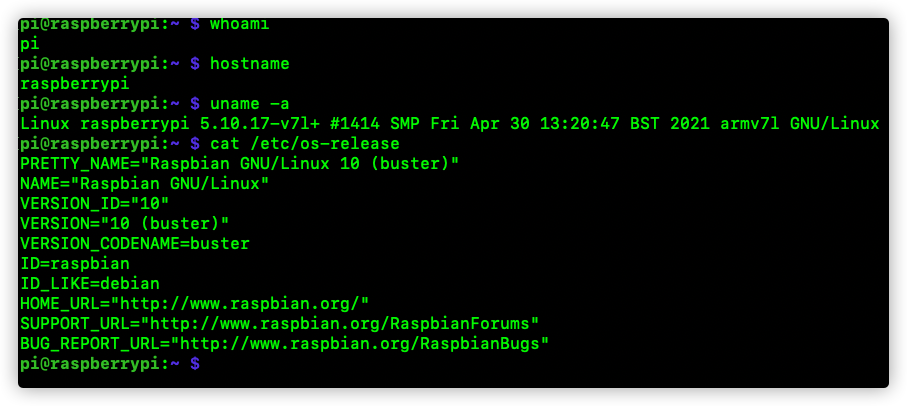
\includegraphics[width=\textwidth, height = 8cm]{img/Figure2.png}
    \centering
    \caption{System Information Result}
    \label{fig:fig2}
\end{figure}
After ensured that the system information was correct, we started customizing the system. According to the manual, we should use the command \code{sudo raspi-config} to change system options, like \textbf{password}, \textbf{hostname} and \textbf{WI-FI},  and localization options, like \textbf{locale}, \textbf{timezone} and \textbf{keyboard}. We thought it would be easy because we had experience configuring Linux systems before, but we didn't expect that we would encounter many problems. Some of them were pretty funny.\par
The first problem was about the WI-FI setting. After we finished the customization of the system and tried to execute the command \code{sudo apt update} to update the Linux kernel, we got wrong message returned which noticed that remote packages resources could not be accessed by this device. This drove us to check our WIFI settings. And then, we found that the SSID we inputted was "\textbf{Redrover}" which should be "\textbf{RedRover}". After fixing the typo and rebooting the system, we were able to execute the command and update the linux kernel without any problems.\par
The next problem is the funny one. When we were setting the local option, we were supposed to unclick the \textbf{"en\_GB.UTF-8 UTF-8"} option and select the \textbf{"en\_us.UTF-8 UTF-8"} option, which represents English. But because of a misreading, we set it to the \textbf{"es\_US.UTF-8 UTF-8"} option, which represents Spanish. However, we didn't know what happened at that time. We just thought the system text became a liitle strange after the reboot, but didn't take much attention on it.\par
Things got even stranger when we started setting up the keyboard. As shown in the manual, we should set the keyboard type as \textbf{"Generic 101 Key PC"}.  Of course we just couldn't find that option as the language had turned to Spanish and none of us was able to understand this situation. So, we asked the professor for help and found that the local setting was the root cause. After fixed this problem, we were able to finish the keyboard setting.\par
The last problem we encountered during configuring the system is the \code{ssh} setting. After confirmed that our Raspberry Pi had connected to the Internet (testing process has mentioned above), we executed the command \code{ifconfig wlan0} for inquiring the IP address. But we failed to connect it with \code{ssh} command. Our first thought is that may be the \code{ssh} command had not been installed yet so we used the command \code{sudo apt install openssh-server} to install the package. But the result noticed that this package had already been installed. Then, we used the command \code{sudo systemctl status ssh} to check the status of the \code{ssh} service. In this way we found the real reason that the \code{ssh} service had not been activated. Once again, we asked the professor for help and he solved this by using the command \code{sudo raspi-config} to enable the \code{ssh} service in the Interface Options. The screenshot of the setting page is shown in figure \ref{fig:fig3}.
\begin{figure}[H]
    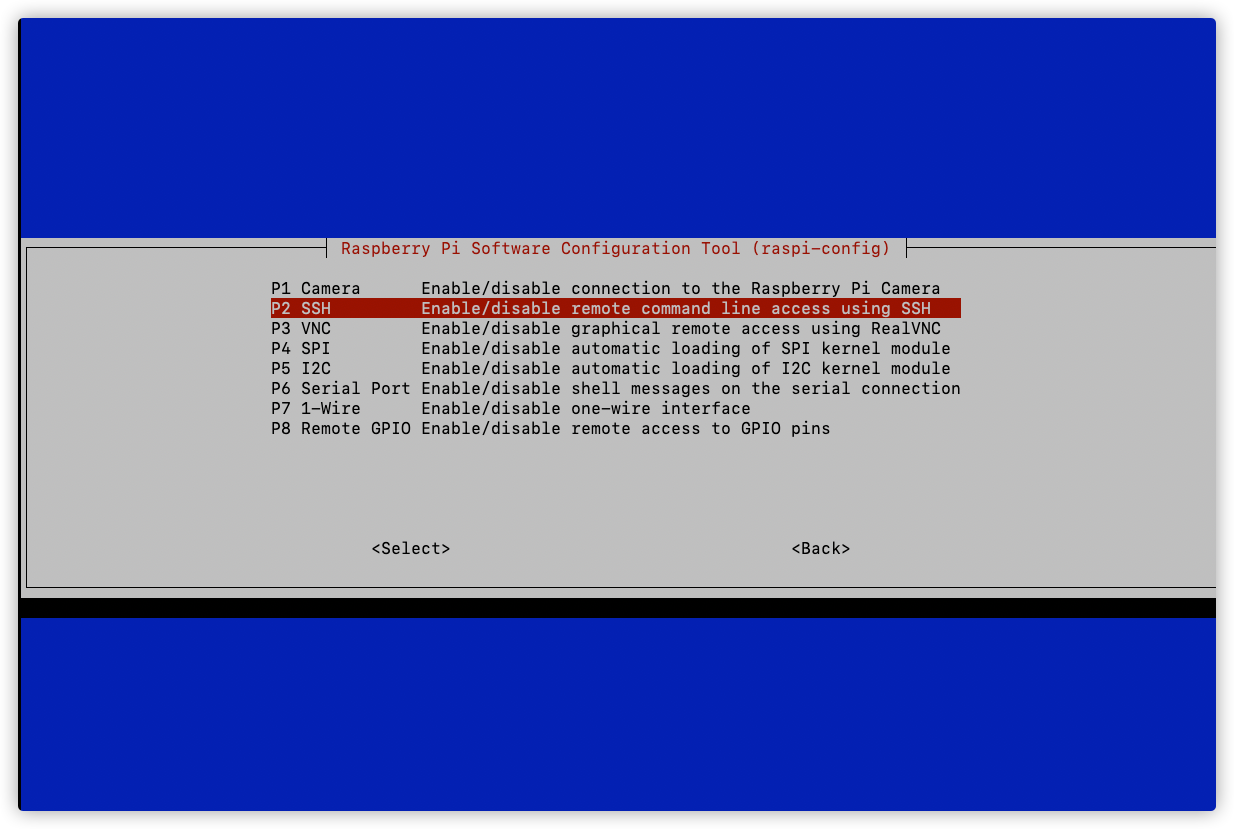
\includegraphics[width=12cm, height = 8cm]{img/Figure3.png}
    \centering
    \caption{SSH Setting Page}
    \label{fig:fig3}
\end{figure}
Finally, we managed to complete the system setup. \vspace{-1em}
\subsection*{2.2 \quad Configure piTFT display and play the video\vspace{-1em}}
In this part, we aimed to setup the piTFT display and play video on it. \par 
The configuration process of the piTFT display went very smoothly and we didn't encounter any problems. The first step was downloading essential packages by the command \code{sudo apt-get} \code{install -y bc fbi git python-pip python-smbus python-spidev evtest libts-bin}.\par
In order to change the boot sequence, we edited the file \code{/boot/config.txt} with \code{vim} and added lines shown in the manual into it. According to the \href{https://www.raspberrypi.org/documentation/computers/config_txt.html}{Raspberry Pi documen}, the \code{/boot/config.txt} stores configuration for booting and will be read it by the early-stage firmware.  The \code{dtoverlay} option make the piTFT be integrated into the boot sequence as an overlay. After edited the \code{/boot/config.txt}, we rebooted the system and observed phenomena that the piTFT screen started out white and then switched to black at the end of boot sequences. Tis phenomena indicated that our initial configuration worked correctly.\par
Then we run the command \code{dmesg} to test if the touch screen of the piTFT was working. The screenshot of similar result is shown in figure \ref{fig:fig4}. (The screenshot was taken when the Raspberry Pi did not connect with HMDI. But it is weird that the chip can not be recognized.)\par
\begin{figure}[H]
    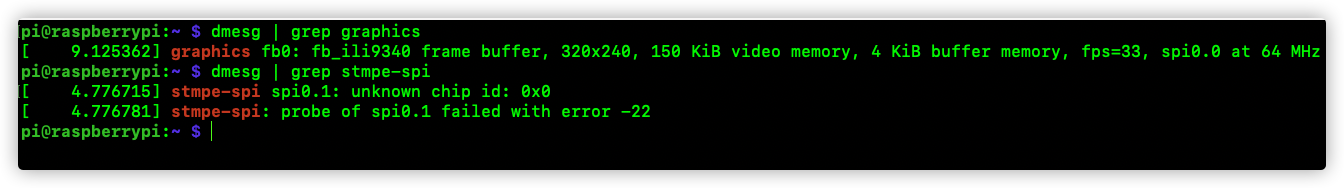
\includegraphics[width=16cm]{img/Figure4.png}
    \centering
    \caption{dmesg result}
    \label{fig:fig4}
\end{figure}
Then, we followed the manual to add a \code{udev} rule by modifying a bunch of files (copy \& paste) and run some commands to stop and restart the touchscreen module. Finally, we could run the command \code{sudo evtest /dev/input/touchscreen} to start testing the touchscreen. The result is shown in figure \ref{fig:fig5}.\par
\begin{figure}[H]
    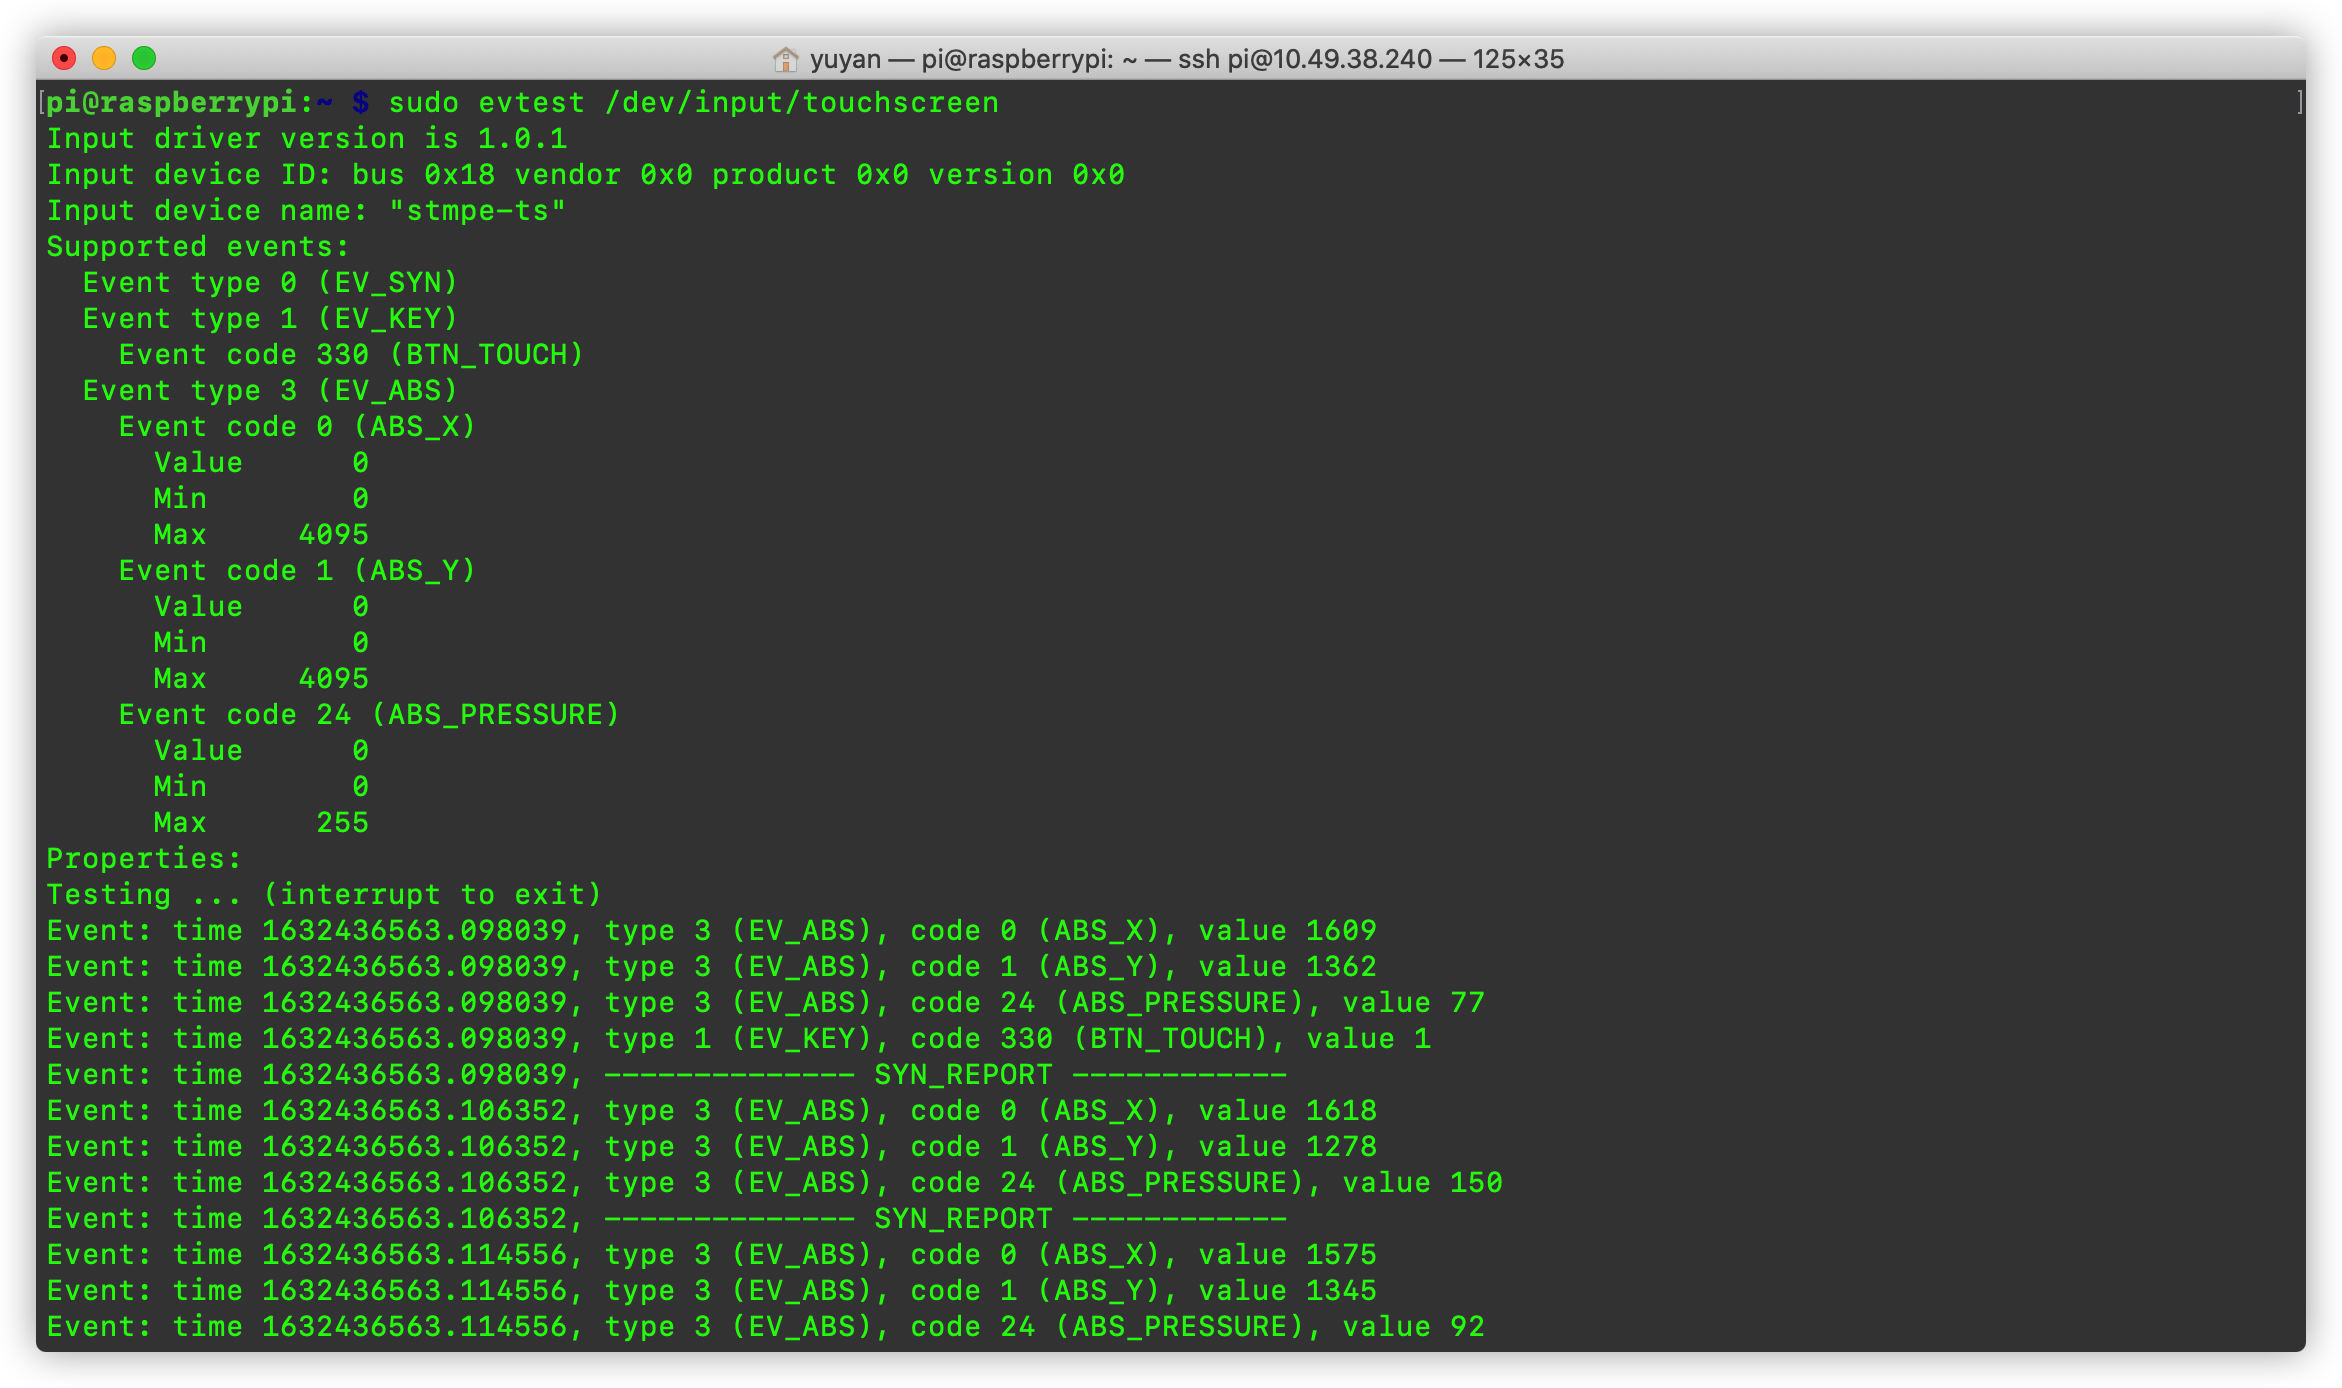
\includegraphics[width=\textwidth]{img/Figure5.png}
    \centering
    \caption{Touchscreen Test}
    \label{fig:fig5}
\end{figure}
After confirmed that the touchscreen could be used normally, we turned to calibrate the piTFT display and then make the Linux console window start on the piTFT by modifying a bunch of files(copy \& paste again). Eventually, we saw the console displayed on the piTFT after the reboot. The result is shown in figure \ref{fig:fig6}.\par
\begin{figure}[H]
    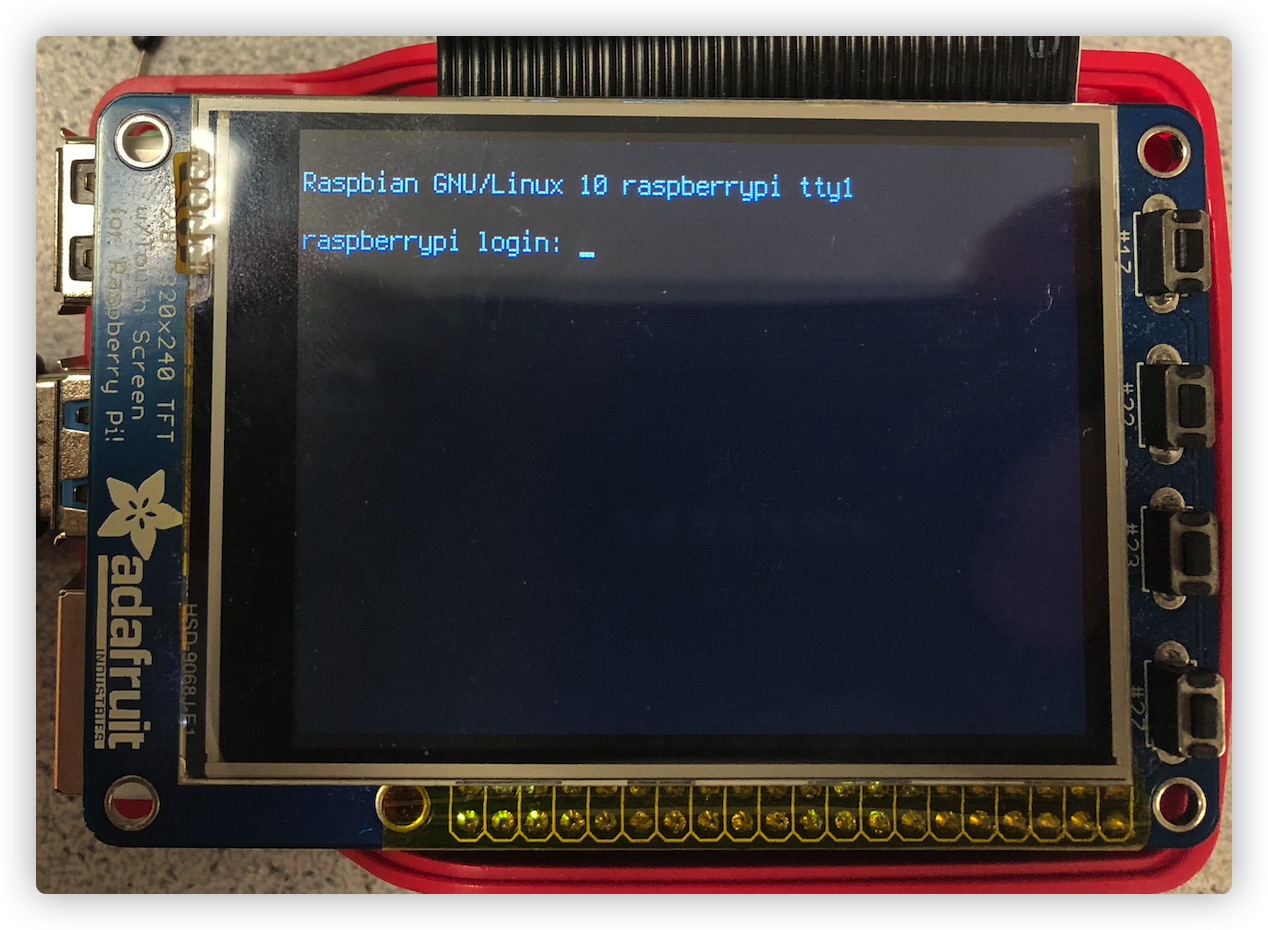
\includegraphics[width=16cm]{img/Figure6.png}
    \centering
    \caption{The terminal on the piTFT}
    \label{fig:fig6}
\end{figure}
We started to check the audio setting and tried to play the video with \code{mylpayer}. We got a JBL speaker from TA and connected it to the Raspberry Pi with an audio cable. Next, we executed the command \code{aplay /usr/share/sounds/alsa/Noise.wav} to test the audio and heard the noise that indicated the audio worked correctly. And then, we used the \code{myplayer} applocation to the video on the different platform, including the piTFT, the monitor and \code{ssh shell} with the command \code{sudo SDL\_VIDEODRIVER=fbcon SDL\_FBDEV=/dev/fb1 mplayer -vo sdl -framedrop} \code{bigbuckbunny320p.mp4} (The option \code{/dev/db1} specifies the playback device which can be looked up by the command \code{ls /dev/fb*}). This command leads us to the most important problem of this part.\par
The root cause of the problem is whether to carry the \code{sudo} option when executing the command. If we run the command with \code{sudo} in the terminal on the piTFT, there would be no sound. Only when we run the command without \code{sudo} will we hear the soud. The situation in the monitor was similar to the piTFT. However, things changed when we run the command through \code{ssh shell}. If we didn't attach the \code{sudo} option in the head of the command, we could only heard the sound without the image of the video. Only if we did attach the \code{sudo} could the video and sound play simultaneously.\par
So at this point, we've successfully deployed piTFT and played the video. Further, we would control the video by pressing the buttons.\par\vspace{-1em}
\subsection*{2.3 \quad Control the video with Python Scripts and the FIFO File\vspace{-1em}}
In this part, we will introduce the experimental process with the main concepts that need to be grasped, and then, focus on describing the only problem we encountered.\par
The experimental process mainly consists of three steps:\vspace{-1em}
\begin{enumerate}
  \item Understand the options of the \code{mplayer} apllication (pause, seek and quit)
  \item Establish the communication between Python scripts and the \code{mplayer} process through the created \code{FIFO} file.
  \item Integrated the GPIO into the Python script for getting input from pressing buttons.
\end{enumerate}\vspace{-1em}

For the step 1, according to the \href{http://www.mplayerhq.hu/DOCS/tech/slave.txt}{reference} in the manual, we found that, in order to fast forward or rewind the video, we should use the \code{seek} option with positive number or negative number (e.g., \code{seek 10} ). The sign of the number determines whether to play forward or backward. As for the quit and pause function, the commands are just as same as their words.\par
For the step2, we created a \code{FIFO} file called \code{video\_fifo} under the home directory. In fact, the \code{FIFo} file works as a pipe which can be leveraged for exchanging messages between different processes. In this specific case, the \code{FIFO} file we created would collect messages sent by the Python process and then deliver them to the \code{mplayer} process. The message generated by the Python script should be like \code{echo "seek 10 " > /home/pi/video\_fifo}. Once this information channel was established, this step had almost been completed.\par
For the last step, we should get the basic understanding of GPIO at first. The full name of GPIO is \textbf{General Purpose Input/Output}. We found the GPIO pins of four buttons on the piTFT  according to the \href{https://canvas.cornell.edu/courses/32456/files/4093447?module_item_id=1105259}{piTFT with R-Pi Schematic}. The result is shown in figure \ref{fig:fig7}.
\begin{figure}[H]
    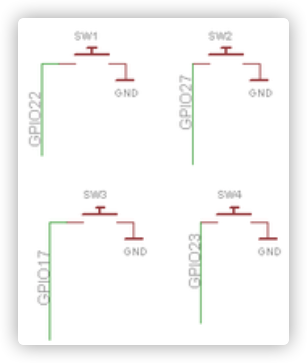
\includegraphics[width=8cm, height=8cm]{img/Figure7.png}
    \centering
    \caption{The terminal on the piTFT}
    \label{fig:fig7}
\end{figure}
Next, we should pay attention to the the Python module  \code{rpi.GPIO}. We mainly used its two functions, \code{setmode} and \code{setup}.
The \code{setmode} funtion is used to set up the numbering system. In this specific case, we setup the numbering system as BCM mode, which refers to the channel numbers on the Broadcom SOC. This is a lower level way and if we change the version of the Raspberry PI, we also need  to change the pin number in our code. And then, we used the \code{setup} function to establish channels for each GPIO pin we used. Through the channel, the input of each button could be connected to the Python process. Once we detected a button was being pressed, the corresponding code would be executed. The complete code is shown in page \pageref{code:5}.\par
To finish the requirements of this part, we still need a bash scrip which could simultaneously run the Python process and the \code{mplayer} process. It was in this step that we ran into the biggest problem. The original version of code is shown in the figure \ref{fig:fig8}.
\begin{figure}[H]
    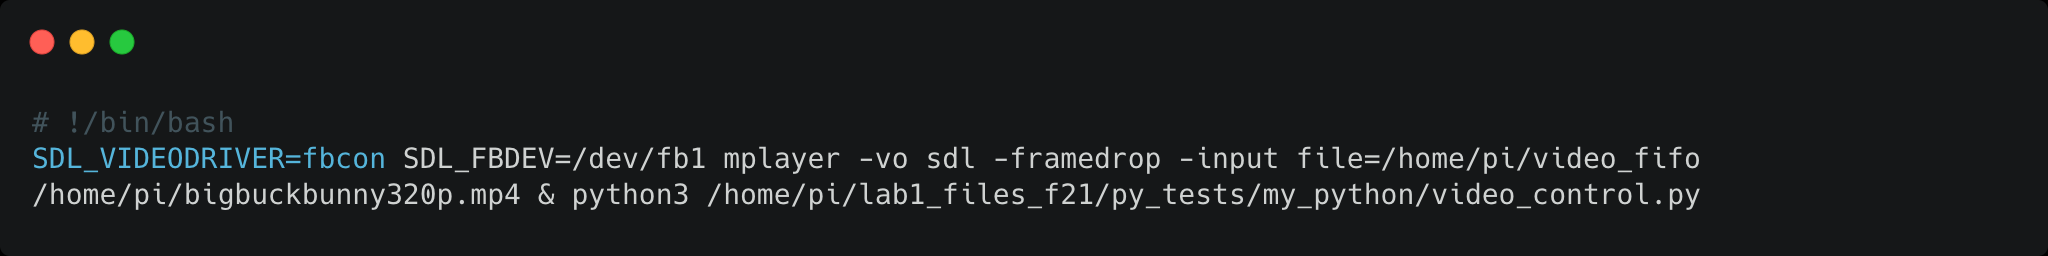
\includegraphics[width=\textwidth]{img/Figure8.png}
    \centering
    \caption{Original Bash Script Code}
    \label{fig:fig8}
\end{figure}
When we demonstrated this script to the TA, we were surprised to find that the \code{myplayer} process did not end automatically when the script process ended. After discussing with the TA, we did not come up with a solution. So, we turned to the professor for help. Of course, the professor figured out this. In our code, we placed the \code{myplayer} process in front and the Python process behind. When we pressed the quit button, it firstly ended the Python process. And then, the bash script was ended. But the \code{myplayer} process was leaved as an orphan process because no one noticed the Linux system to end it. So, it would get stuck there, not knowing what to do, until we forced it to stop by pressing \code{ctrl-c}.\par
The solution to fix this problem is really easy. Just switch their position. In this case, after the quit button pressed, the Python process would end. And then, it would trigger the end of the bash script which would also end the \code{myplayer} process. The correct version of the code is shown in Figure \ref{fig:fig9}.\par
\begin{figure}[H]
    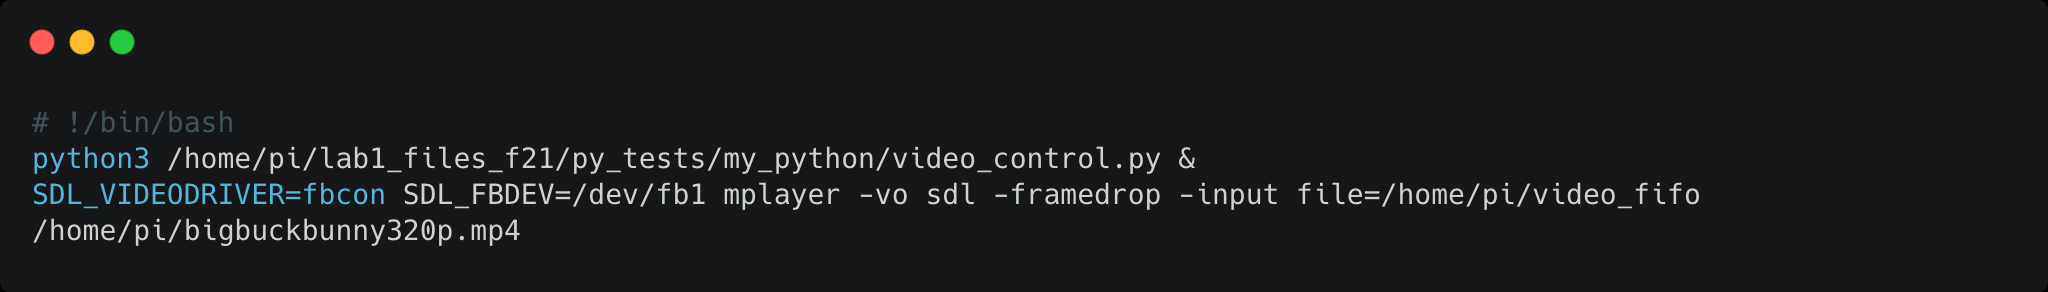
\includegraphics[width=\textwidth]{img/Figure9.png}
    \centering
    \caption{Correct Version of Bash Script Code}
    \label{fig:fig9}
\end{figure}
\newpage
\section*{3. Conclusions\vspace{-1em}}
In this Lab1, we have successfully completed all the parts with good results (the first team passed).\par
The configuration process for the Raspberry Pi was a lot more convoluted than we expected. However, the complexity of scripts is still within our capacity. Thus, considering the overall workload of the two-week experiment, we would suggest that the workload of the second week could be increased as Python coding involved in this section should be a bit too basic for the students in this class. Personally, I (Yu Zhang) would like to suggest that principle for modifying the boot sequence and other configuration processes could be clearer. Most students, including us, just copied and pasted the commands and configurations from the lab manual. Even though they finished the experiment smoothly, they may still own limited understanding with the Linux system. \par
The biggest insight we obtained from the whole experiment is that the Linux system is a highly customizable system. Even the boot sequence can be modified at user's will. Of course, users should own the access rights of the super admin. This also places additional demands on the user, requiring a higher level of operating system and programming knowledge background. No wonder that the Linux system has remained viable for so long and is always the dominant operating system in industry. \par
The most surprising result I got is the process ending sequence mention in page \pageref{fig:fig8}. I never thought there would be a time when a process would be orphaned and stuck. This also shows the high tolerance of the Linux system. As the professor said in the class, the Linux system will always execute what you have executed. Be Careful! But \textbf{Don't Panic}. The worst case is to start all over again. So, Remember to Make the \textbf{Backup}!\par
Overall, I think this is a very good start experiment for this course. Not only do we get a first glance at the Linux system, but also we can appreciate the Raspberry Pi's charm. It only costs \$35 to support most computer functions with the Linux system installed. At last, we must solemnly thank all the \textbf{TAs} and \textbf{Prof. Skovira} for all the help they provided during the experiment.\par

\newpage
\section*{4. Code Appendix\vspace{-1em}}
\textbf{1. fifo\_test.py}
\begin{lstlisting}[language=Python]
# Yu Zhang yz2729
# Xinyu Wu xw586
# Lab 1  Date: 09/16/21
import subprocess
import os
while True:
    # Get inpu from the user
    command = input("Please input a command: ")
    print(command)
    if command == "pause":
        # Pause
        cmd = 'echo "pause" > /home/pi/video_fifo'
        os.system(cmd)
    elif command == "get_file_name":
        # Get File Name
        cmd = 'echo "get_file_name" > /home/pi/video_fifo'
        os.system(cmd)
    elif command == "speed_set":
        # Speed Up
        cmd = 'echo "speed_set 10" > /home/pi/video_fifo'
        os.system(cmd)
    elif command == "quit":
        # Quit
        cmd = 'echo "quit" > /home/pi/video_fifo'
        os.system(cmd)
        break
print("The viedo is end!")
\end{lstlisting}
\textbf{2. one\_button.py}
\begin{lstlisting}[language=Python]
# Yu Zhang yz2729
# Xinyu Wu xw586
# Lab 1  Date: 09/16/21
import RPi.GPIO as GPIO
import os
import time
# Set Numbering System to BCM mode
GPIO.setmode(GPIO.BCM)
# Setup the GPIO channel
GPIO.setup(17, GPIO.IN, pull_up_down=GPIO.PUD_UP)

while True:
    time.sleep(0.2)
    # Detect input
    if(not GPIO.input(17)):
        print("Button 17 has been pressed")
\end{lstlisting}

\newpage
\textbf{3. four\_button.py}
\begin{lstlisting}[language=Python]
# Yu Zhang yz2729
# Xinyu Wu xw586
# Lab 1  Date: 09/16/21
import RPi.GPIO as GPIO
import os
import time
# Set Numbering System to BCM mode
GPIO.setmode(GPIO.BCM)
# Setup the GPIO channel
GPIO.setup(17, GPIO.IN, pull_up_down=GPIO.PUD_UP)
GPIO.setup(22, GPIO.IN, pull_up_down=GPIO.PUD_UP)
GPIO.setup(23, GPIO.IN, pull_up_down=GPIO.PUD_UP)
GPIO.setup(27, GPIO.IN, pull_up_down=GPIO.PUD_UP)
while True:
    time.sleep(0.2)
    if(not GPIO.input(17)):
        print("Button 17 has been pressed")
    elif( not GPIO.input(22)):
        print("Button 22 has been pressed")    
    elif( not GPIO.input(23)):
        print("")
        print("Button 23 has been pressed")
    elif( not GPIO.input(27)):
        print("")
        print("Button 27 has been pressed")
        break
\end{lstlisting}

\textbf{4. start\_video.sh}
\begin{lstlisting}[language=Bash]
# !/bin/bash
# Yu Zhang yz2729
# Xinyu Wu xw586
# Lab 1  Date: 09/16/21
python3 /home/pi/lab1_files_f21/py_tests/my_python/video_control.py &
SDL_VIDEODRIVER=fbcon SDL_FBDEV=/dev/fb1 mplayer -vo sdl -framedrop -input file=/home/pi/video_fifo /home/pi/bigbuckbunny320p.mp4
\end{lstlisting}

\newpage
\textbf{5. video\_control.py} \label{code:5}
\begin{lstlisting}[language=Python] 
# Yu Zhang yz2729
# Xinyu Wu xw586
# Lab 1  Date: 09/16/21
import RPi.GPIO as GPIO
import os
import time
# Set Numbering System to BCM mode
GPIO.setmode(GPIO.BCM)
# Setup the GPIO channel
GPIO.setup(17, GPIO.IN, pull_up_down=GPIO.PUD_UP)
GPIO.setup(22, GPIO.IN, pull_up_down=GPIO.PUD_UP)
GPIO.setup(23, GPIO.IN, pull_up_down=GPIO.PUD_UP)
GPIO.setup(27, GPIO.IN, pull_up_down=GPIO.PUD_UP)
while True:
    time.sleep(0.2)
    if(not GPIO.input(17)):
        # Pause
        print("Button 17 has been pressed")
        cmd = 'echo "pause" > /home/pi/video_fifo'
        print("Pause the Video")
        os.system(cmd)
    elif( not GPIO.input(22)):
        # Fast Forward
        print("Button 22 has been pressed") 
        cmd = 'echo "seek 10 " > /home/pi/video_fifo'
        print("Fast forward 10 seconds")
        os.system(cmd)
    elif( not GPIO.input(23)):
        # Rewind
        print("Button 23 has been pressed")
        cmd = 'echo "seek -10" > /home/pi/video_fifo'
        print("Rewind 10 seconds")
        os.system(cmd)
    elif( not GPIO.input(27)):
        # Quit
        print("Button 27 has been pressed")
        cmd = 'echo "quit" > /home/pi/video_fifo'
        print("Quit the Video")
        os.system(cmd)
        break
\end{lstlisting}
% To add math, use
%\begin{equation}
 %Helpful links    https://www.overleaf.com/learn/latex/Mathematical_expressions
%\end{equation}

%To add hyperlinks, use 
%For further references see \href{http://www.overleaf.com}{Something Linky} or go to the next url: \url{http://www.overleaf.com}

% It's also possible to link directly any word or \hyperlink{thesentence}{any sentence} in you document.

% Tables 

% \begin{table}[h!]
% \centering
%  \begin{tabular}{||c c c c||} 
%  \hline
%  Col1 & Col2 & Col2 & Col3 \\ [0.5ex] 
%  \hline\hline
%  1 & 6 & 87837 & 787 \\ 
%  2 & 7 & 78 & 5415 \\
%  3 & 545 & 778 & 7507 \\
%  4 & 545 & 18744 & 7560 \\
%  5 & 88 & 788 & 6344 \\ [1ex] 
%  \hline
%  \end{tabular}
% \end{table}

% Images

% upload your images to the img folder. To print them in the document, uncomment the following
% \begin{figure}[h]
%     \centering
%     \includegraphics[width=0.25\textwidth]{/img/YourImageTitle}
%     \caption{a nice plot}
%     \label{fig:mesh1}
% \end{figure}

% As you can see in the figure \ref{fig:mesh1}, the 
% function grows near 0. Also, in the page \pageref{fig:mesh1} 
% is the same example.
\newpage
\printbibliography

\end{document}
